\chapter{Work Object Data}
\label{ch:workobject}
\markboth{Work Object Data}{}

\begin{flushright}
	{\smaller
		\textit{It is not certain\\ that everything is uncertain}\\
		-- Blaise Pascal}
\end{flushright}

All the following analysis will be carried out using a default aircraft. This choice is made in order to avoid the collection and validation data phase for each analysis and make focus on the results. As mentioned, there are two default aircraft in the code: ATR-72 and Boieng 747-100B whose data are shown in the table below.\\
All the analyses that follow, refer to the data presented in this chapter and those derived from them .



%
\begingroup
\begin{longtable}[h]{lll}
\textbf{} & \textbf{ATR-72} & \textbf{B747-100B}\\
\toprule
\endfirsthead
%
\multicolumn{3}{l}%
  {\relsize{-1}({\itshape continued from previous page})}\\
\textbf{} & \textbf{ATR-72} & \textbf{B747-100B}\\
\toprule
\endhead
%
\midrule \multicolumn{3}{r}{{\relsize{-1}\itshape continued on next page}}
\endfoot
%
\bottomrule
\caption{ATR-72 and B747-100B input data}
\endlastfoot
%
\textbf{Operating Conditions} & \textbf{} & \textbf{}\\
\midrule
Altitude & $\SI{6000.0000}{\meter}$ & $\SI{10000.0000}{\meter}$ \\
Cruising Mach number & 0.4300 &  0.8300 \\
\midrule
\textbf{Weights} & \textbf{ } & \textbf{ }\\
\midrule
Maximum Take-Off Mass & $\SI{23063.5790}{\kilogram}$ & $\SI{354991.5060}{\kilogram}$ \\
Operating Empty Mass & $\SI{12935.5790}{\kilogram}$ & $\SI{153131.9860}{\kilogram}$\\
Maximum Fuel Mass & $\SI{5000.0000}{\kilogram}$ & $\SI{147409.5200}{\kilogram}$ \\
Maximum number of passengers & 72 & 550 \\
\midrule
\textbf{Fuselage} & \textbf{ } & \textbf{ }\\
\midrule
Length & $\SI{27.1660}{\meter}$ & $\SI{68.6300}{\meter}$ \\
Diameter & $\SI{2.7561}{\meter}$ & $\SI{6.7934}{\meter}$ \\
Fineness Ratio & 9.8566 & 10.1025  \\
\midrule
\textbf{Wing} & \textbf{ } & \textbf{ }\\
\midrule
Surface & $\SI{61.0000}{\square\meter}$  & $\SI{511.0000}{\square\meter}$ \\
\AR & 12.0000 & 6.9000 \\
Span & $\SI{27.05549}{\meter}$ & $\SI{59.3792}{\meter}$ \\
Taper Ratio & 0.5450 & 0.2840 \\
Root Chord & $\SI{2.9186}{\meter}$ & $\SI{14.6152}{\meter}$ \\
Mean Aerodynamic Chord & $\SI{2.3198}{\meter}$ & $\SI{9.6913}{\meter}$ \\
Sweep\textsubscript{LE} & $\SI{2.8390}{\degree}$ & $\SI{38.4290}{\degree}$\\
Sweep\textsubscript{C/4} & $\SI{1.3997}{\degree}$ & $\SI{35.4999}{\degree}$ \\
$t/c_{\text{max}}$ & 0.1675 & 0.1292 \\
$C_{D0}$ & 0.03170  & 0.01820 \\
Oswald Factor & 0.7585 & 0.6277 \\
Airfoil type & Conventional & Modern Supercritical\\
\midrule
\textbf{Horizontal Tail} & \textbf{ } & \textbf{ }\\
\midrule
Surface & $\SI{11.7300}{\square\meter}$  & $\SI{136.6000}{\square\meter}$\\
\AR & 4.5550  & 3.5700\\
Span & $\SI{7.3095}{\meter}$  & $\SI{22.08307}{\meter}$\\
Taper Ratio & 0.5700 & 0.2650\\
Root Chord & $\SI{2.04430}{\meter}$ & $\SI{9.7798}{\meter}$\\
Mean Aerodynamic Chord & $\SI{1.6450}{\meter}$ & $\SI{6.8835}{\meter}$\\
Sweep\textsubscript{LE} & $\SI{3.4410}{\degree}$ & $\SI{38.2250}{\degree}$\\
Sweep\textsubscript{C/4} & $\SI{0.0000}{\degree}$ & $\SI{32.0003}{\degree}$\\
$t/c_{\text{max}}$ & 0.1500 & 0.1500\\
\midrule
\textbf{Vertical Tail} & \textbf{ } & \textbf{ }\\
\midrule
Surface & $\SI{12.4800}{\square\meter}$ & $\SI{77.1000}{\square\meter}$\\
\AR &  1.6600 & 1.3400\\
Span & $\SI{4.5515}{\meter}$ & $\SI{10.1643}{\meter}$\\
Taper Ratio & 0.3200 & 0.3300 \\
Root Chord & $\SI{4.1544}{\meter}$ & $\SI{11.4065}{\meter}$\\
Mean Aerodynamic Chord & $\SI{2.9323}{\meter}$ & $\SI{8.2285}{\meter}$\\
Sweep\textsubscript{LE} & $\SI{40.5485}{\degree}$  & $\SI{53.9913}{\degree}$\\
Sweep\textsubscript{C/4} & $\SI{28.5998}{\degree}$  & $\SI{45.0001}{\degree}$ \\
$t/c_{\text{max}}$ & 0.2227 & 0.2245 \\
\midrule
\textbf{Power Plant} & \textbf{ } & \textbf{ }\\
\midrule
Static Thrust (per engine) & $\SI{7700.0000}{\newton}$ & $\SI{204000.0000}{\newton}$\\
Engines Number & 2 & 4\\
Engines type & Turboprop & Turbofan\\
BRR & 0.0000 & 5.0000\\
$\eta_{\text{p}}$ & 0.85 & 0.00 \\
\end{longtable}
\endgroup


\begin{figure}[H]
\centering
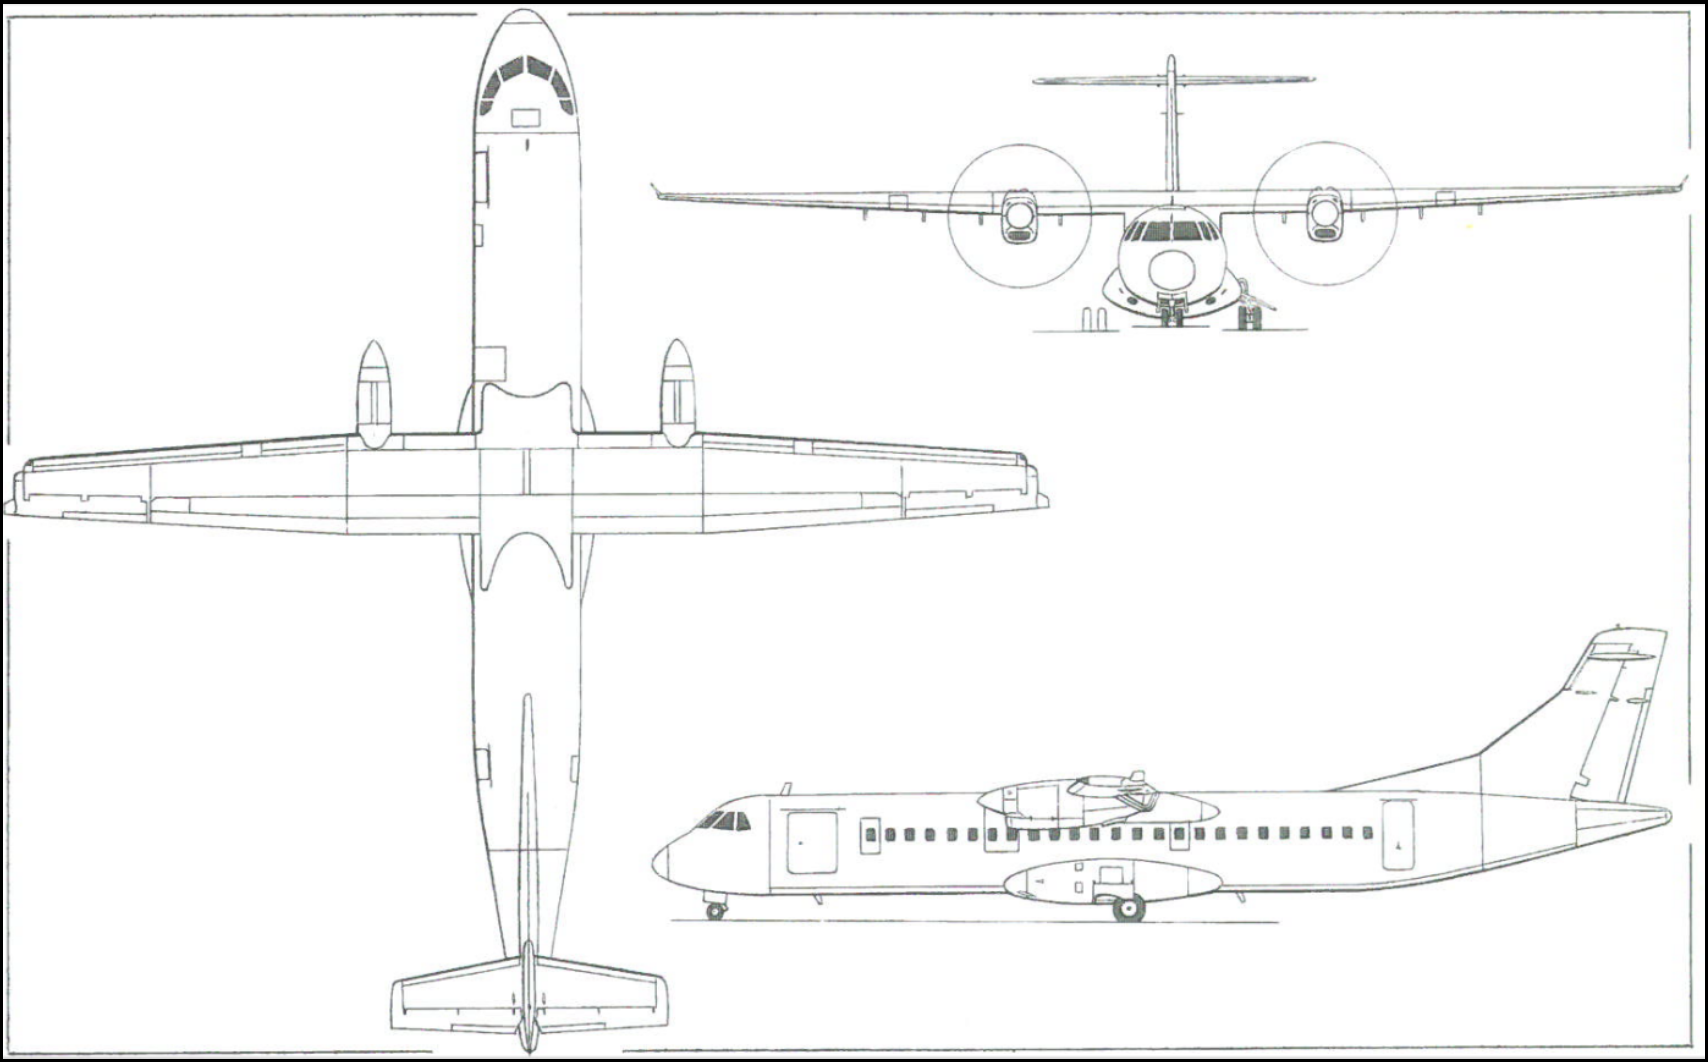
\includegraphics[height=6.4cm]{Immagini/ATR-72}
\caption{ATR-72 views – Jane’s All the World’s Aircraft 2004-2005.}
\label{atr}
\end{figure}
\begin{figure}[H]
\centering
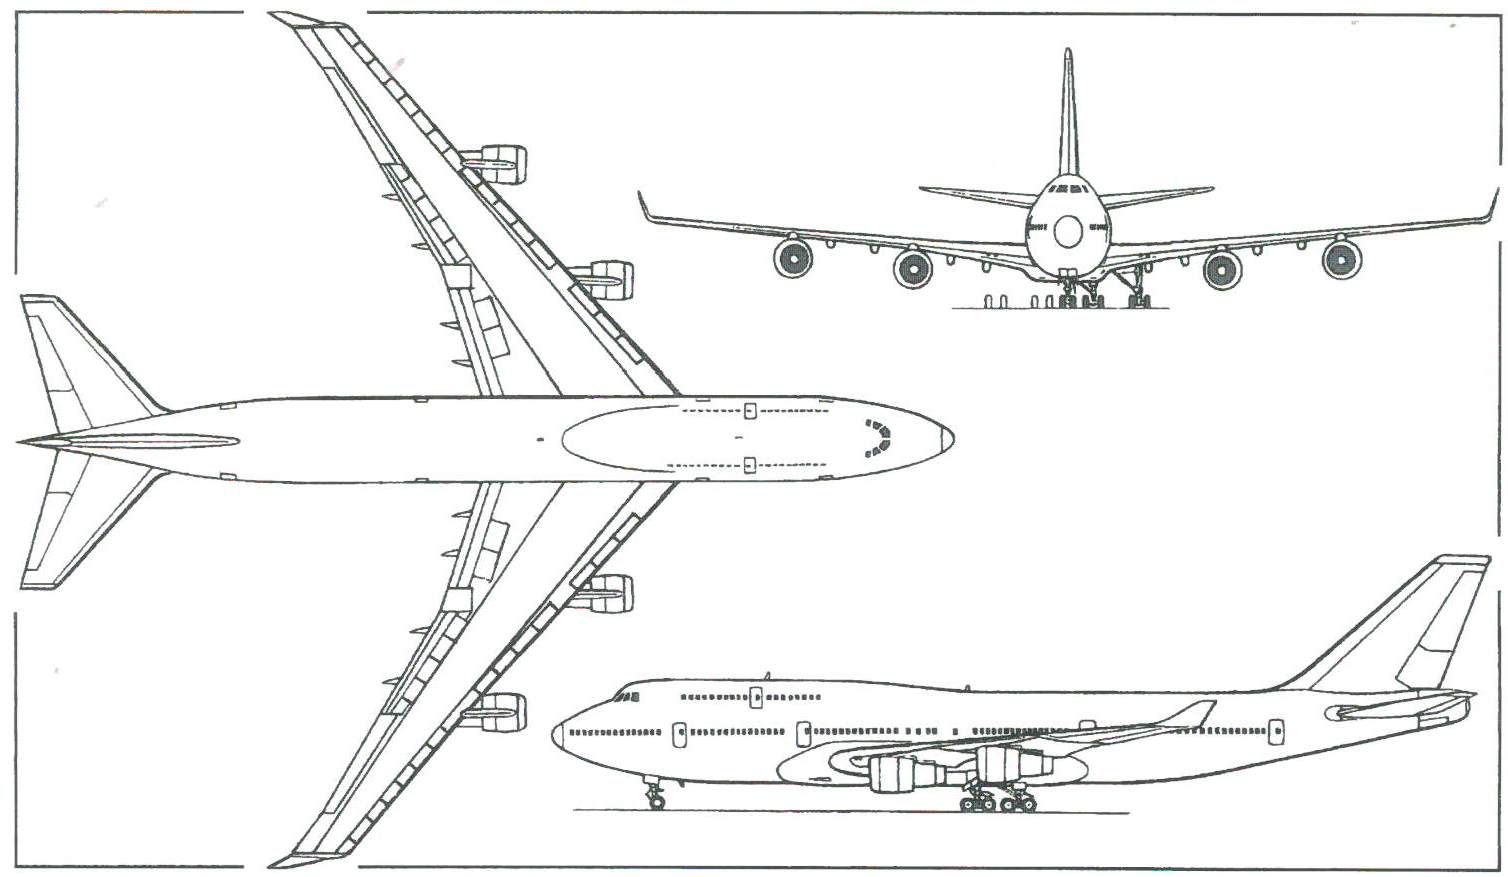
\includegraphics[height=6.4cm]{Immagini/B747-100B}
\caption{B747-100B views – Jane’s All the World’s Aircraft 2004-2005.}
\label{boeing}
\end{figure}